\subsection{Utilisation d'un joystick}
	Le jeu permet l'utilisation jusqu'à quatre joysticks simultanément. Si vous souhaitez utiliser un joystick, veuillez le brancher avant le lancement du jeu pour une meilleur recognition.
	
\subsection{Utilisation d'une wiimote}

	L'utilisation d'une wiimote nécessite d'avoir un périphérique bluetooth sur l'ordinateur. Celui peut-être intégré à l'ordinateur, si ce n'est pas le cas, vous pouvez utiliser une clé usb bluetooth. Une liste des périphériques compatibles se trouve à cette \href{http://wiibrew.org/wiki/List_of_Working_Bluetooth_Devices}{adresse}, pour information nous avons utilisé le modèle \textit{Trendnet TBW-105UB} lors du développement de ce jeu.
	
	
	Lors du lancement de l'application, l'écran suivant vous invite à brancher les wiimotes. Comme pour le joystick, l'application ne peut gérer plus de quatre wiimotes.
	
\begin{figure}[h]
	\begin{center}
		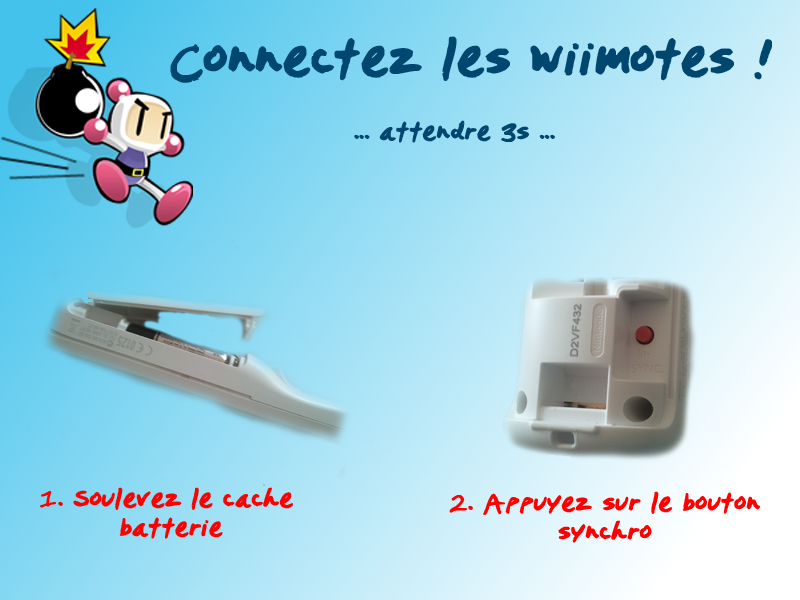
\includegraphics[scale=0.5]{images/wiiScreen.png}
		\caption{Ecran de connexion des wiimotes}
	\end{center}
\end{figure}

		
	Vous avez à ce moment là trois secondes pour brancher les wiimotes que vous souhaitez utiliser, en suivant les indications à l'écran.
	

\subsection{Utilisation du clavier}

L'utilisation du clavier ne nécessite aucune action de votre part. Dans le cas où aucun joystick ou wiimotes ne sont branchés, le clavier est défini comme contrôleur de jeu par défaut pour tous les joueurs.
